\documentclass[12pt]{beamer}

\usepackage{tikz}
\usepackage{graphicx}
\usepackage[T1]{fontenc}
\usepackage{amsmath}
\usepackage{multicol}
\usetikzlibrary{graphs, graphs.standard}

\DeclareMathOperator{\E}{\textrm{E}}		     % expected value
\DeclareMathOperator{\pr}{\mathrm{P}}		     % probability 
\DeclareMathOperator{\cov}{t_{cov}}	             % cover time

\title{Cover Times of Random Walks}
\author{R. Teal Witter}
\institute{Middlebury College}
\date{May 9, 2019}

\begin{document}

\frame{\titlepage}

\begin{frame}{Overview}
\tableofcontents
\end{frame}

\AtBeginSection[]
{
  \begin{frame}<beamer>
    \frametitle{Overview}
    \tableofcontents[currentsection]
  \end{frame}
}

\section{Introduction}

\begin{frame} \only<1>{\frametitle{A Graph}}

\only<2->{\frametitle{Random Walks}}

\centering
\begin{center}
	\begin{tikzpicture}[scale=.9] [
        > = stealth, % arrow head style
        shorten > = 1pt, % don't touch arrow head to node
        %auto,
        node distance = 3cm, % distance between nodes
        semithick % line style
    ]

		\tikzstyle{edge}=[draw,line width = .5pt,-,black!100]

		\node (m) at (0,0) {
			\begin{tikzpicture}[scale = 3]
			    \tikzstyle{edge}=[draw,line width = .5pt,-,black!100]
			    \tikzstyle{current}=[draw,circle,fill=black,scale=.5]
			    \tikzstyle{visited}=[draw,circle,fill=white,scale=.5]
			    \draw[edge] (0,0) -- (0,1);
			    \draw[edge] (0,0) -- (1,0);
			    \draw[edge] (0,1) -- (1,0);
			    \draw[edge] (0,1) -- (1,1);
			    \draw[edge] (1,1) -- (1,0);
			    \node (bl) at (0,0) {};
			    \node[current] (tl) at (0,1) {};
			    \only<1>{\node[current] (2) at (1,1) {};}
		        \only<1>{\node[current] (3) at (1,0) {};}
		        \only<1>{\node[current] (4) at (0,0) {};}
			    \node (br) at (1,0) {};
			    \node (tr) at (1,1) {};;
			\end{tikzpicture}
		};
		\pause
		\pause
		\node (a) at (4,3) {
			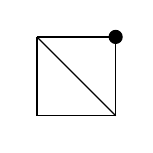
\begin{tikzpicture}[scale = 1]
			    \tikzstyle{edge}=[draw,line width = .5pt,-,black!100]
			    \tikzstyle{current}=[draw,circle,fill=black,scale=.5]
			    \tikzstyle{visited}=[draw,circle,fill=white,scale=.5]
			    \draw[edge] (0,0) -- (0,1);
			    \draw[edge] (0,0) -- (1,0);
			    \draw[edge] (0,1) -- (1,0);
			    \draw[edge] (0,1) -- (1,1);
			    \draw[edge] (1,1) -- (1,0);
			    \node (bl) at (0,0) {};
			    \node[current] (br) at (1,1) {};
			    \node (tr) at (1,1) {};;
			\end{tikzpicture}
		};
		\node (b) at (4,0) {
			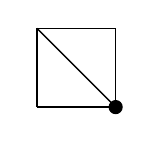
\begin{tikzpicture}[scale = 1]
			    \tikzstyle{edge}=[draw,line width = .5pt,-,black!100]
			    \tikzstyle{current}=[draw,circle,fill=black,scale=.5]
			    \tikzstyle{visited}=[draw,circle,fill=white,scale=.5]
			    \draw[edge] (0,0) -- (0,1);
			    \draw[edge] (0,0) -- (1,0);
			    \draw[edge] (0,1) -- (1,0);
			    \draw[edge] (0,1) -- (1,1);
			    \draw[edge] (1,1) -- (1,0);
			    \node (bl) at (0,0) {};
			    \node (br) at (1,0) {};
			    \node[current] (tr) at (1,0) {};;
			\end{tikzpicture}
		};
	    \node (c) at (4,-3) {
			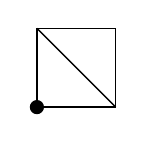
\begin{tikzpicture}[scale = 1]
			    \tikzstyle{edge}=[draw,line width = .5pt,-,black!100]
			    \tikzstyle{current}=[draw,circle,fill=black,scale=.5]
			    \tikzstyle{visited}=[draw,circle,fill=white,scale=.5]
			    \draw[edge] (0,0) -- (0,1);
			    \draw[edge] (0,0) -- (1,0);
			    \draw[edge] (0,1) -- (1,0);
			    \draw[edge] (0,1) -- (1,1);
			    \draw[edge] (1,1) -- (1,0);
			    \node (bl) at (0,0) {};
			    \node[current] (tr) at (0,0) {};;
			\end{tikzpicture}
		};
		\path[->] (m) edge (a);
		\path[->] (m) edge (b);
		\path[->] (m) edge (c);
		\pause
		\path[->] (m) edge node[above] {$\frac{1}{3}$} (a);	
	    \path[->] (m) edge node[below] {$\frac{1}{3}$} (b); 
	    \path[->] (m) edge node[below] {$\frac{1}{3}$} (c); 
	\end{tikzpicture}
\end{center}
\end{frame}

\begin{frame}{Cover Times}
\centering
How many steps does a random walk take to visit every vertex?
\end{frame}

\begin{frame}{Coupon Collector}
\centering
A collector receives one of $n$ possible coupons in the mail everyday.
How long until all $n$ coupons have been collected?
\end{frame}

\begin{frame}{Birthday Problem}
\centering
How many people do we need for each birthday (excluding February 29)
to be represented?
\end{frame}

\section{Expected Cover Time of a Small Graph}

\begin{frame}{A Small Graph}
\centering
\begin{center}
	\begin{tikzpicture}[scale=.9] [
        > = stealth, % arrow head style
        shorten > = 1pt, % don't touch arrow head to node
        %auto,
        node distance = 3cm, % distance between nodes
        semithick % line style
    ]

		\tikzstyle{edge}=[draw,line width = .5pt,-,black!100]

		\node (m) at (-1.2,1.75) {
			\begin{tikzpicture}[scale = 3]
			    \tikzstyle{edge}=[draw,line width = .5pt,-,black!100]
			    \tikzstyle{current}=[draw,circle,fill=black,scale=.5]
			    \tikzstyle{visited}=[draw,circle,fill=white,scale=.5]
			    \draw[edge] (0,0) -- (0,1);
			    \draw[edge] (0,0) -- (1,0);
			    \draw[edge] (0,1) -- (1,0);
			    \draw[edge] (0,1) -- (1,1);
			    \draw[edge] (1,1) -- (1,0);
%			    \node (l) at (.5, 1.1) {$\cov$};
			    \node (bl) at (0,0) {};
			    \node[current] (tl) at (0,1) {};
			    \node (br) at (1,0) {};
			    \node (tr) at (1,1) {};;
			\end{tikzpicture}
		};
		\pause

		\node (a) at (2,3) {
			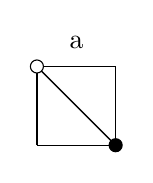
\begin{tikzpicture}[scale = 1]
			    \tikzstyle{edge}=[draw,line width = .5pt,-,black!100]
			    \tikzstyle{current}=[draw,circle,fill=black,scale=.5]
			    \tikzstyle{visited}=[draw,circle,fill=white,scale=.5]
			    \draw[edge] (0,0) -- (0,1);
			    \draw[edge] (0,0) -- (1,0);
			    \draw[edge] (0,1) -- (1,0);
			    \draw[edge] (0,1) -- (1,1);
			    \draw[edge] (1,1) -- (1,0);
			    \node (l) at (.5, 1.3) {a};
			    \node (bl) at (0,0) {};
			    \node[visited] (tl) at (0,1) {};
			    \node[current] (br) at (1,0) {};
			    \node (tr) at (1,1) {};;
			\end{tikzpicture}
		};
		\node (b) at (2,0) {
			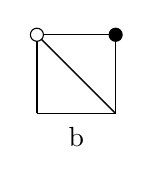
\begin{tikzpicture}[scale = 1]
			    \tikzstyle{edge}=[draw,line width = .5pt,-,black!100]
			    \tikzstyle{current}=[draw,circle,fill=black,scale=.5]
			    \tikzstyle{visited}=[draw,circle,fill=white,scale=.5]
			    \draw[edge] (0,0) -- (0,1);
			    \draw[edge] (0,0) -- (1,0);
			    \draw[edge] (0,1) -- (1,0);
			    \draw[edge] (0,1) -- (1,1);
			    \draw[edge] (1,1) -- (1,0);
			    \node (l) at (.5, -.3) {b};
			    \node (bl) at (0,0) {};
			    \node[visited] (tl) at (0,1) {};
			    \node (br) at (1,0) {};
			    \node[current] (tr) at (1,1) {};;
			\end{tikzpicture}
		};
		\path[->] (m) edge (a);
		\path[->] (m) edge (b);
		\pause
		\node (c) at (4,3) {
			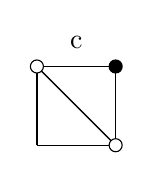
\begin{tikzpicture}[scale = 1]
			    \tikzstyle{edge}=[draw,line width = .5pt,-,black!100]
			    \tikzstyle{current}=[draw,circle,fill=black,scale=.5]
			    \tikzstyle{visited}=[draw,circle,fill=white,scale=.5]
			    \draw[edge] (0,0) -- (0,1);
			    \draw[edge] (0,0) -- (1,0);
			    \draw[edge] (0,1) -- (1,0);
			    \draw[edge] (0,1) -- (1,1);
			    \draw[edge] (1,1) -- (1,0);
			    \node (l) at (.5, 1.3) {c};
			    \node (bl) at (0,0) {};
			    \node[visited] (tl) at (0,1) {};
			    \node[visited] (br) at (1,0) {};
			    \node[current] (tr) at (1,1) {};;
			\end{tikzpicture}
		};
		\node (d) at (4,0) {
			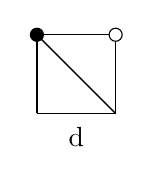
\begin{tikzpicture}[scale = 1]
			    \tikzstyle{edge}=[draw,line width = .5pt,-,black!100]
			    \tikzstyle{current}=[draw,circle,fill=black,scale=.5]
			    \tikzstyle{visited}=[draw,circle,fill=white,scale=.5]
			    \draw[edge] (0,0) -- (0,1);
			    \draw[edge] (0,0) -- (1,0);
			    \draw[edge] (0,1) -- (1,0);
			    \draw[edge] (0,1) -- (1,1);
			    \draw[edge] (1,1) -- (1,0);
			    \node (l) at (.5, -.3) {d};
			    \node (bl) at (0,0) {};
			    \node[current] (tl) at (0,1) {};
			    \node (br) at (1,0) {};
			    \node[visited] (tr) at (1,1) {};;
			\end{tikzpicture}
		};
		\node (e) at (6,3) {
			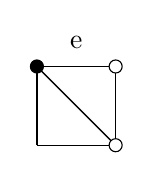
\begin{tikzpicture}[scale = 1]
			    \tikzstyle{edge}=[draw,line width = .5pt,-,black!100]
			    \tikzstyle{current}=[draw,circle,fill=black,scale=.5]
			    \tikzstyle{visited}=[draw,circle,fill=white,scale=.5]
			    \draw[edge] (0,0) -- (0,1);
			    \draw[edge] (0,0) -- (1,0);
			    \draw[edge] (0,1) -- (1,0);
			    \draw[edge] (0,1) -- (1,1);
			    \draw[edge] (1,1) -- (1,0);
			    \node (l) at (.5, 1.3) {e};
			    \node (bl) at (0,0) {};
			    \node[current] (tl) at (0,1) {};
			    \node[visited] (br) at (1,0) {};
			    \node[visited] (tr) at (1,1) {};;
			\end{tikzpicture}
		};		
		\path[->] (a) edge[loop above, distance=6mm] (a);
		\path[->] (a) edge (c);
		\path[->] (b) edge[bend left] (d);
		\path[->] (b) edge (e);
		\pause
		\node (f) at (6, 0) {
			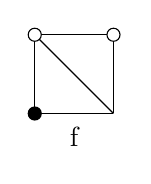
\begin{tikzpicture}[scale = 1]
			    \tikzstyle{edge}=[draw,line width = .5pt,-,black!100]
			    \tikzstyle{current}=[draw,circle,fill=black,scale=.5]
			    \tikzstyle{visited}=[draw,circle,fill=white,scale=.5]
			    \draw[edge] (0,0) -- (0,1);
			    \draw[edge] (0,0) -- (1,0);
			    \draw[edge] (0,1) -- (1,0);
			    \draw[edge] (0,1) -- (1,1);
			    \draw[edge] (1,1) -- (1,0);
			    \node (l) at (.5, -.3) {f};
			    \node[current] (bl) at (0,0) {};
			    \node[visited] (tl) at (0,1) {};
			    \node (br) at (1,0) {};
			    \node[visited] (tr) at (1,1) {};;
			\end{tikzpicture}
		};
		\node (done) at (8, 3) {
			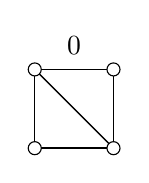
\begin{tikzpicture}[scale = 1]
			    \tikzstyle{edge}=[draw,line width = .5pt,-,black!100]
			    \tikzstyle{current}=[draw,circle,fill=black,scale=.5]
			    \tikzstyle{visited}=[draw,circle,fill=white,scale=.5]
			    \draw[edge] (0,0) -- (0,1);
			    \draw[edge] (0,0) -- (1,0);
			    \draw[edge] (0,1) -- (1,0);
			    \draw[edge] (0,1) -- (1,1);
			    \draw[edge] (1,1) -- (1,0);
			    \node (l) at (.5, 1.3) {0};
			    \node[visited] (bl) at (0,0) {};
			    \node[visited] (tl) at (0,1) {};
			    \node[visited] (br) at (1,0) {};
			    \node[visited] (tr) at (1,1) {};;
			\end{tikzpicture}
		};
		\node (g) at (8, 0) {
			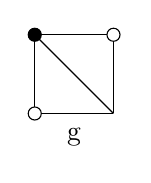
\begin{tikzpicture}[scale = 1]
			    \tikzstyle{edge}=[draw,line width = .5pt,-,black!100]
			    \tikzstyle{current}=[draw,circle,fill=black,scale=.5]
			    \tikzstyle{visited}=[draw,circle,fill=white,scale=.5]
			    \draw[edge] (0,0) -- (0,1);
			    \draw[edge] (0,0) -- (1,0);
			    \draw[edge] (0,1) -- (1,0);
			    \draw[edge] (0,1) -- (1,1);
			    \draw[edge] (1,1) -- (1,0);
			    \node (l) at (.5, -.3) {g};
			    \node[visited] (bl) at (0,0) {};
			    \node[current] (tl) at (0,1) {};
			    \node (br) at (1,0) {};
			    \node[visited] (tr) at (1,1) {};;
			\end{tikzpicture}
		};
		\path[->] (c) edge[bend left] (e);
		\path[->] (d) edge (e);
		\path[->] (d) edge[bend left] (b);
		\path[->] (d) edge (f);
		\path[->] (e) edge[bend left] (c);
		\path[->] (e) edge[loop above, distance=6mm] (e);
		\path[->] (f) edge[bend left] (g);
		\path[->] (g) edge[bend left] (f);
		\path[->] (e) edge (done);
		\path[->] (f) edge (done);
		\path[->] (g) edge (done);
	\end{tikzpicture}
\end{center}
\end{frame}

\begin{frame}{A Small Graph}
\small
\begin{align}
\E[\cov] &= 1 + \frac{1}{3}\textrm{a} + \frac{2}{3}\textrm{b} 
\only<2->{= \frac{43}{6}}\nonumber \\
\textrm{a} &= 1 + \frac{1}{3}\textrm{a} + \frac{2}{3}\textrm{c} \nonumber \\
\textrm{b} &= 1 + \frac{1}{2}\textrm{b} + \frac{1}{2}\textrm{e} \nonumber \\
\textrm{c} &= 1 + 1\textrm{e} \nonumber \\
\textrm{d} &= 1 + \frac{1}{3}\textrm{a} + \frac{1}{3}\textrm{e} + \frac{1}{3}\textrm{f} \nonumber \\
\textrm{e} &= 1 + \frac{1}{3}\textrm{c} + \frac{1}{3}\textrm{e} + \frac{1}{3} 0\nonumber \\
\textrm{f} &= 1 + \frac{1}{2}\textrm{g} + \frac{1}{2} 0 \nonumber \\
\textrm{g} &= 1 + \frac{2}{3}\textrm{f} + \frac{1}{3} 0\nonumber
\end{align}
\end{frame}

\section{Expected Cover Time of a Complete Graph with Self-edges}

\begin{frame}{Complete Graph with Self-edges}
Let $X_i$ be the number of steps from $i-1$ to $i$ distinct vertices.
\only<2-> {
\begin{align}
\E[\cov] &= \E[X_1+X_2+X_3+\cdots+X_{n}] \nonumber
\end{align}
}

\only<3-> {$X_i \sim \textrm{Geom}(\frac{n-i+1}{n})$}
\only<4-> {so $\E[X_i] = \frac{n}{n-i+1}$}
\only<5-> {and
\begin{align}
\E[\cov] &= n\left(\frac{1}{n}+\frac{1}{n-1}+\cdots+1\right) \nonumber
\end{align}
}
\end{frame}

\begin{frame}{Coupon Collector}
\centering
A collector receives one of $n$ possible coupons in the mail everyday.
How long until all coupons have been collected?
\bigskip

On average, we need about $n \log n$ days.
\end{frame}

\begin{frame}{Birthday Problem}
\centering
How many people do we need for each birthday (excluding February 29)
to be represented?
\bigskip

On average, we need about 2365 people.
\end{frame}

\section{Expected Cover Time of a General Graph}

\begin{frame}{Matthews Method}
\begin{theorem}
Consider a random walk on an arbitrary connected graph with $n$ vertices. Then
\end{theorem}
\begin{align}
\E[\cov] &\leq t_{hit} \left(1 + \frac{1}{2} + \frac{1}{3} + \cdots + \frac{1}{n-1} \right). \nonumber
\end{align}
\end{frame}

\begin{frame}{Matthews Method Proof}
Let $\sigma$ be a uniform permutation of unvisited vertices from (worst-case) vertex $n$.
\pause

Let $T_k$ be the first time vertices 
$\sigma_1, \sigma_2, \ldots, \sigma_k$ have all been visited.
\pause
\begin{align}
\E[\cov] &= \E_n[{T_{n-1}}]  \nonumber \\
&\leq \E_n[T_1 + (T_2 - T_1) + \cdots + (T_{n-1} - T_{n-2})] \nonumber
\end{align}


\end{frame}
\begin{frame}{Matthews Method Proof}

Let $L(k)$ be the final vertex to be visited among 
$\sigma_1, \sigma_2, \ldots, \sigma_k$ before the first time they are
all visited.
\pause
\begin{align}
\E_n[T_k - T_{k-1}] &=
\sum_{i=1}^k \E_n[T_k - T_{k-1} | L(k) = \sigma_i]
\pr(L_k = \sigma_i) \nonumber
\only<3->{\\&= 0 +
\E_n[T_k - T_{k-1} | L(k) = \sigma_k]
\pr(L_k = \sigma_k) \nonumber 
}
\only<4->{\\&\leq t_{hit} \frac{1}{k} \nonumber }
\end{align}
\end{frame}

\section{Cover Time Distribution of the a Complete Graph with Self-edges}

\begin{frame}{Cover Time Distribution}
After $r$ steps of a random walk, let $A_i$ be the event that
vertex $i$ is unvisited.
\begin{align}
\pr(A_i) = \pr(\textrm{not visited in one step})^r = (1-1/n)^r \nonumber
\end{align}
\pause
Let $N_n$ be the number of unvisited vertices.
\begin{align}
\E[N_n] &= \sum_{i=1}^n \pr(A_i) = n(1-1/n)^r \nonumber  \\
&=n[(1-1/n)^n]^{r/n} \sim n e^{-r/n} \nonumber
\end{align}

\end{frame}

\begin{frame}{Cover Time Distribution}
Introduce $x$ and set $r = n \log n + nx$.
\begin{align}
N_n &\sim ne^{-r/n} = ne^{-\log n - x} = n n^{-1} e^{-x} \rightarrow  e^{-x} \nonumber
\end{align}
\begin{theorem}
If $ne^{-r/n} \rightarrow \lambda \in [0, \infty)$, then the number of unvisited
vertices approaches a Poisson distribution with mean $\lambda$.
\end{theorem}
\pause
\begin{align}
\pr(N_n=0) = \pr(\cov \leq r)
= \pr(\cov - n \log n\leq nx)
\rightarrow e^{-e^{-x}} \nonumber
\end{align}
\end{frame}

\begin{frame}{Birthday Problem}
What is the probability all birthdays are covered in a town of 1825?
How about a town of 2190?
\pause
\begin{align}
\pr(\cov \leq 1825) &= \pr \left(\frac{\cov - 2153}{365} \leq
\frac{-328}{365}\right) \nonumber \\
&\approx e^{-e^{-0.89863}} \approx 0.08576 \nonumber
\only<3->{
\\\pr(\cov \leq 2190) &= \pr \left(\frac{\cov - 2153}{365} \leq
\frac{37}{365}\right) \nonumber \\
&\approx e^{-e^{-0.10137}} \approx 0.40511 \nonumber
}
\end{align}

\end{frame}

\begin{frame}{Birthday Problem}
\begin{tikzpicture}[scale=.37]
\node (graph) at (0,0) {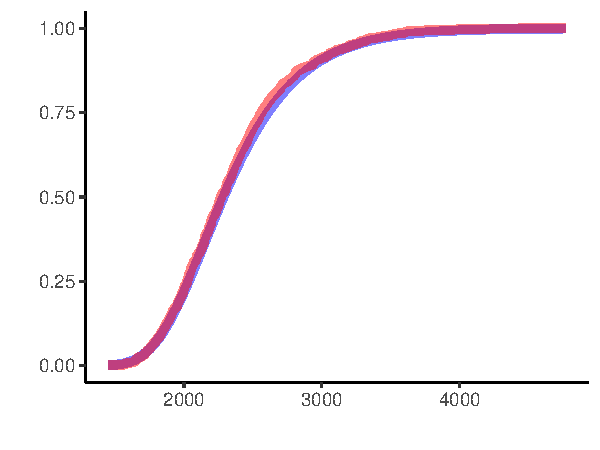
\includegraphics[scale=.1, height=7cm]{birthdays}};
\node (title) at (1, 10) {Cover Times of the Birthday Problem (1000 trials)};
\node[rotate=90] (ylabel) at (-13,2) {$\pr(\cov \leq r)$};
\node (xlabel) at (0,-9) {$r$};
\end{tikzpicture}
\end{frame}

\begin{frame}{Thank you!}
\centering
github.com/rtealw/Cover-Times
\medskip
\begin{thebibliography}{9}

\bibitem{AF14}
	Aldous, D. and J. Fill.
	2014.
	\textit{Reversible Markov Chains and Random Walks on Graphs}.

\bibitem{BH94}
	Blom, G., L. Holst and D. Sandell.
	\textit{Problems and Snapshots from the World of Probability},
	Springer Science \& Business Media, 1994.

\bibitem{DS84}
	Doyle, P. G. and J. L. Snell.
	1984.
	\textit{Random Walks and Electric Networks},
	Mathematical Association of America.
 
\bibitem{LP08}
	Levin, D. A. and Y. Peres.
	2017.
	\textit{Markov Chains and Mixing Times},
	Vol. 107,
	American Mathematical Society.

\end{thebibliography}
\end{frame}

\end{document}

























